\section{Pricing dimension: empirical sensitivity and statistical identification}

\subsection{Development-period dimension surfaces}

Within the original diagnostic family, the preferred dimension changes with the data definition and pricing geometry (Figure~\ref{fig:dev-surfaces}). Each row is a candidate dimension within one feature-lineage--test-asset environment, and each column is one of the 21 evaluation geometries. Cell color measures the percentage pricing-distance loss relative to the pointwise best candidate, so the figure preserves both the winner and the economic size of every model's shortfall. The outlined path follows the winner based on the five-seed mean, while circle size records how many individual seeds select that row. A single model does not dominate every asset family and every geometry. For Core-86, the aggregate endpoint winner for the combined 74 assets moves from $K=2$ under the equal-moment endpoint to $K=4$ under the HJ endpoint. The industry and size--book-to-market sets move from $K=2$ to $K=1$. For Core-92, the equal-moment endpoint selects $K=5$ for all three primary sets, while the HJ endpoint selects $K=1$, $4$, and $8$ for the combined, industry, and size--book-to-market assets.

\begin{widefigure}[!tbp]
\centering
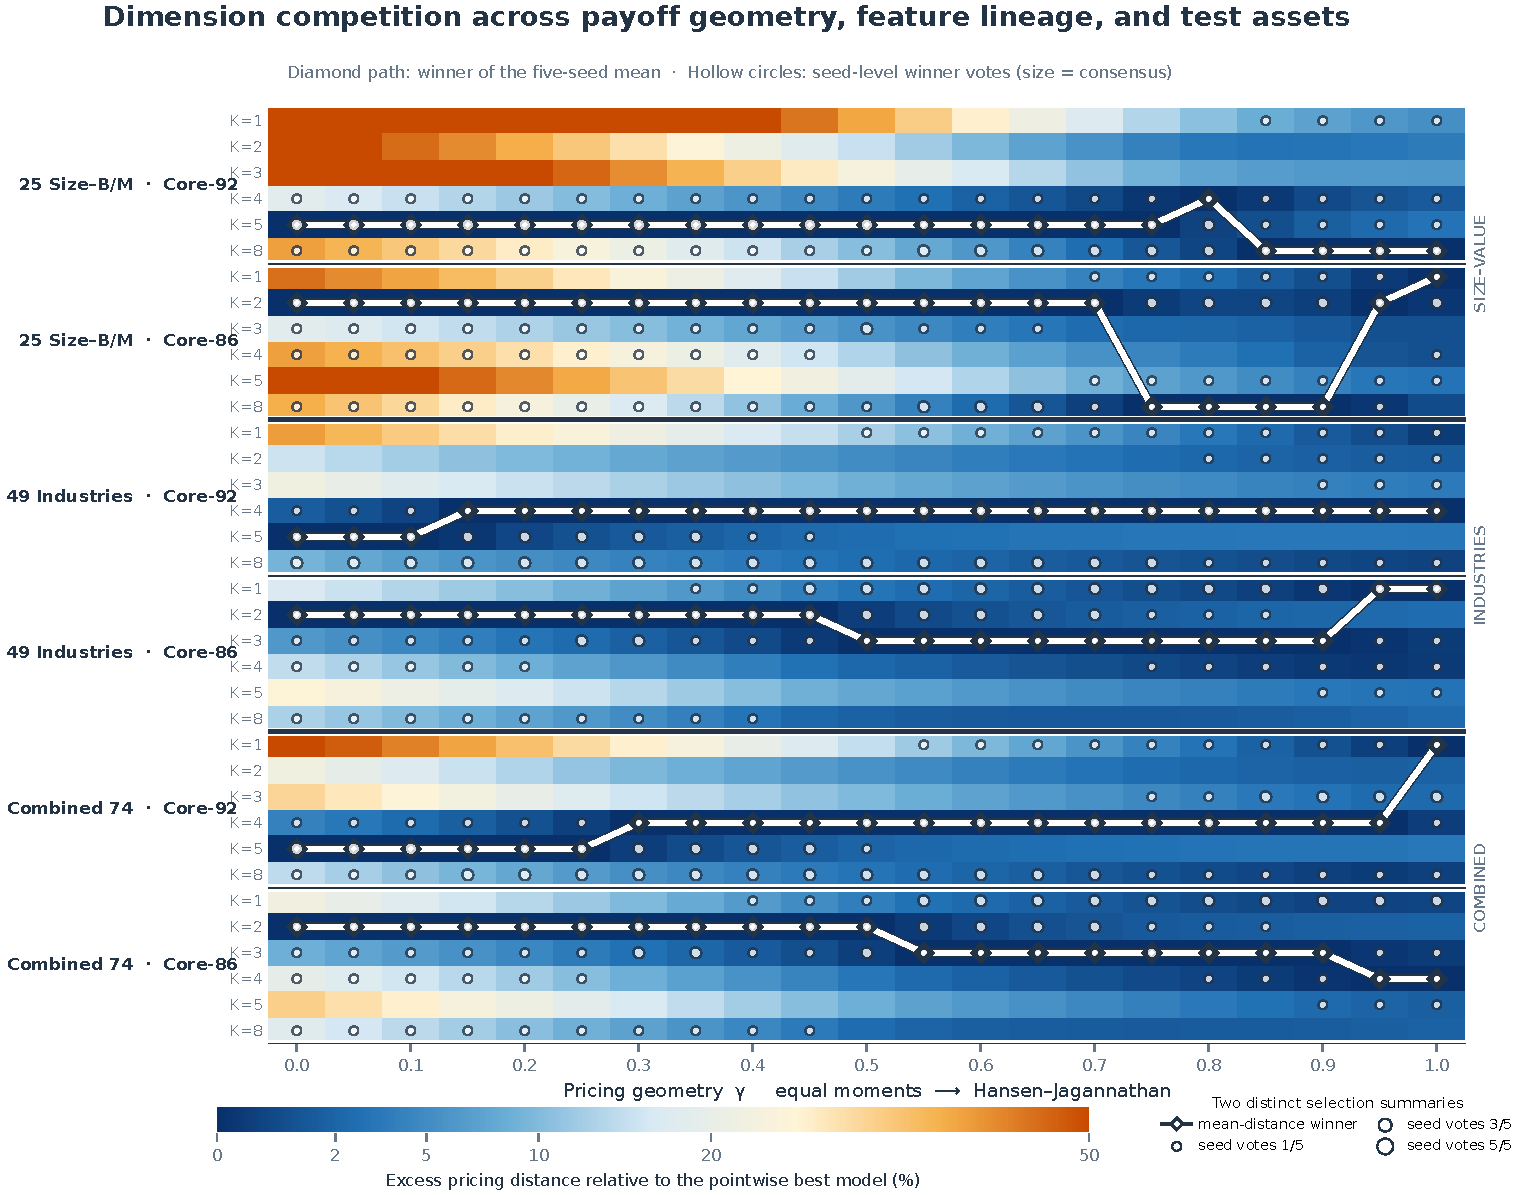
\includegraphics[width=0.98\textwidth]{figure_02_dimension_sensitivity.pdf}
\caption{Empirical dimension-competition field. The 756 cells report every frozen five-seed mean for the archived development windows: two characteristic definitions, three primary test-asset sets, six candidate dimensions, and 21 evaluation geometries. Color is excess pricing distance relative to the best candidate in the same environment and geometry, clipped at 50\% for display; dark blue denotes close competition and orange denotes economically large shortfall. The outlined diamond path follows the winner of the five-seed mean. Hollow circles are a distinct statistic: their area records one to five seed-level winner votes for the corresponding dimension, computed from all 3,780 seed-specific distances. A circle away from the diamond path therefore indicates seed-level support that does not win after averaging. Geometry zero is the equal-moment endpoint and one is the HJ-type endpoint. Core-92 evaluates February 2010--January 2020 returns; Core-86 evaluates January 2010--December 2019 returns. The comparison also changes construction and coverage, not only feature count.}
\label{fig:dev-surfaces}
\end{widefigure}

Table~\ref{tab:dimension-evidence} reports all six candidate dimensions at both endpoints. Its common column structure allows a direct comparison of Core-92 and Core-86 within each asset set. Boldface identifies the seed-mean minimum; neighboring entries show whether that minimum is separated from the alternatives. Parentheses summarize dispersion across five fixed training seeds, not time-series sampling uncertainty.

\begin{widetable}[!tbp]
\centering
\begin{minipage}{\textwidth}
\caption{Pricing distances for every candidate dimension, archived development windows}
\label{tab:dimension-evidence}
\footnotesize
\setlength{\tabcolsep}{4pt}
\renewcommand{\arraystretch}{1.16}
\begin{tabular*}{\linewidth}{@{\extracolsep{\fill}}crrrr@{}}
\toprule
 & \multicolumn{2}{c}{Core-92} & \multicolumn{2}{c}{Core-86} \\
\cmidrule(lr){2-3}\cmidrule(l){4-5}
$K$ & Equal moments & HJ & Equal moments & HJ \\
\midrule
\multicolumn{5}{@{}l}{\textit{A. 25 size--book-to-market portfolios}} \\[2pt]
$1$ & 3.321 (0.183) & 1.840 (0.022) & 2.365 (0.105) & \textbf{1.841} (0.038) \\
$2$ & 2.455 (0.219) & 1.809 (0.036) & \textbf{1.633} (0.143) & 1.843 (0.037) \\
$3$ & 2.725 (0.306) & 1.856 (0.070) & 1.935 (0.167) & 1.858 (0.024) \\
$4$ & 1.893 (0.205) & 1.771 (0.050) & 2.269 (0.391) & 1.857 (0.024) \\
$5$ & \textbf{1.597} (0.314) & 1.798 (0.041) & 2.564 (0.315) & 1.895 (0.054) \\
$8$ & 2.221 (0.336) & \textbf{1.746} (0.047) & 2.236 (0.325) & 1.854 (0.023) \\
\addlinespace[5pt]
\multicolumn{5}{@{}l}{\textit{B. 49 industry portfolios}} \\[2pt]
$1$ & 4.305 (0.126) & 2.332 (0.030) & 3.465 (0.137) & \textbf{2.306} (0.054) \\
$2$ & 3.566 (0.201) & 2.363 (0.048) & \textbf{2.964} (0.130) & 2.365 (0.042) \\
$3$ & 3.771 (0.326) & 2.411 (0.080) & 3.151 (0.117) & 2.311 (0.061) \\
$4$ & 3.137 (0.217) & \textbf{2.328} (0.041) & 3.394 (0.276) & 2.310 (0.044) \\
$5$ & \textbf{3.088} (0.207) & 2.403 (0.041) & 3.718 (0.251) & 2.376 (0.084) \\
$8$ & 3.371 (0.285) & 2.337 (0.041) & 3.348 (0.212) & 2.360 (0.061) \\
\addlinespace[5pt]
\multicolumn{5}{@{}l}{\textit{C. Combined 74 portfolios}} \\[2pt]
$1$ & 5.410 (0.199) & \textbf{2.802} (0.025) & 4.208 (0.168) & 2.750 (0.041) \\
$2$ & 4.343 (0.277) & 2.854 (0.042) & \textbf{3.438} (0.177) & 2.790 (0.033) \\
$3$ & 4.651 (0.433) & 2.867 (0.073) & 3.735 (0.177) & 2.743 (0.055) \\
$4$ & 3.706 (0.277) & 2.808 (0.034) & 4.115 (0.421) & \textbf{2.738} (0.032) \\
$5$ & \textbf{3.559} (0.308) & 2.895 (0.033) & 4.535 (0.362) & 2.785 (0.069) \\
$8$ & 4.067 (0.403) & 2.811 (0.035) & 4.058 (0.324) & 2.788 (0.049) \\
\bottomrule
\end{tabular*}
\par\vspace{4pt}
{\footnotesize\raggedright\textit{Notes:} Each entry is a mean pricing distance over five fixed training seeds; parentheses give the standard error across seeds. Lower is better. Boldface marks the smallest mean within each asset set, data definition, and loss geometry. Seed standard errors describe algorithmic dispersion, not time-series sampling uncertainty. Core-92 return months are February 2010--January 2020; Core-86 return months are January 2010--December 2019. Construction and coverage also differ. All six candidates are shown, including those that never win.\par}
\end{minipage}
\end{widetable}


The result is not merely that two losses produce two answers. The economic content of a pricing error depends on direction. Equal weighting emphasizes the coordinate representation of the moments. HJ weighting discounts directions with large payoff second moments and emphasizes directions that are expensive to span. If weak priced directions are correlated with dominant common directions, a change in $W$ changes the signal-to-noise tradeoff. A dimension claim that is robust only to one geometry is therefore a statement about that loss, not a loss-free risk count.

\subsection{Data-definition and seed instability}

The archived Core-92 and Core-86 row blocks in Figure~\ref{fig:dev-surfaces}, together with Table~\ref{tab:dimension-evidence}, compare the entire six-dimension ordering under the two feature lineages. Exact agreement is nearly absent. Across 21 geometries, the best $K$ agrees twice for the 25 size--book-to-market portfolios, never for industries, and once for the combined assets. Mean Spearman correlations are $-0.355$, $-0.156$, and $-0.151$, respectively; their minima are $-0.600$, $-0.371$, and $-0.371$. Mean Kendall correlations are $-0.263$, $-0.111$, and $-0.124$. The color field also shows that the result is not uniformly driven by economically negligible ties: some switches occur within a broad blue region of small descriptive loss gaps, while others coincide with large orange shortfalls for the displaced candidate. Thus the change reaches beyond a close tie at the minimum; it reverses much of the ordering.

This archived comparison cannot separate feature information from measurement, coverage, missingness, and timing. We therefore retain it as a pipeline sensitivity result and examine deletion separately using the later same-panel control. Neither comparison identifies the marginal causal effect of an individual characteristic on expected returns.

Seed sensitivity points in the same direction. There are 12 combinations of data definition, primary asset set, and endpoint geometry. None yields a five-of-five unanimous best dimension. Averaging across seeds is a useful performance summary, but it does not make the underlying structural object seed-invariant. The distinction is analogous to model averaging: aggregation can stabilize a prediction while leaving model selection uncertain.

\subsection{What survives a same-panel feature ablation?}

The controlled comparison is less disruptive than the archived pipeline contrast. Keeping rows, return months, ranks, input positions, and paired initialization fixed produces mean rank correlations of 0.649 for size--book-to-market portfolios, 0.722 for industries, and 0.703 for the combined assets across the 21 geometries. Winner agreement occurs in 9, 9, and 11 geometries, respectively. Thus some exact minima still switch, but deleting the six features alone does not reproduce the broad negative rank correlations of the two archived pipelines in this design.

For the combined 74 assets, both full and masked arms select $K=4$ under equal moments and $K=5$ under the HJ-type endpoint. Table~\ref{tab:matched-features} retains all fixed-$K$ comparisons rather than reporting only those winners. Under the HJ-type endpoint the $K=5$ distance is 2.700 with all features and 2.699 after masking, a difference of $-0.0007$ with interval $[-0.0600,0.0700]$. All six HJ-endpoint paired intervals include zero. Under equal moments, masking raises the $K=1$ distance by 0.3855 with pointwise interval $[0.0172,0.9277]$; the remaining five intervals include zero. This single exclusion of zero among twelve primary intervals is not familywise evidence of a general feature effect.

\begin{widetable}[!tbp]
\centering
\begin{minipage}{\textwidth}
\caption{Matched six-feature ablation: pricing distances and paired uncertainty}
\label{tab:matched-features}
\footnotesize
\setlength{\tabcolsep}{4pt}
\renewcommand{\arraystretch}{1.16}
\begin{tabular*}{\linewidth}{@{\extracolsep{\fill}}crrrrc@{}}
\toprule
$K$ & Full 92 & Masked 86 & Difference & 95\% interval & $K^*$ frequency \\
\midrule
\multicolumn{6}{@{}l}{\textit{A. Equal-moment endpoint}} \\[2pt]
1 & 5.227 & 5.612 & +0.385 & [0.017, 0.928] & 0.0 / 0.0 \\
2 & 4.449 & 3.980 & -0.469 & [-1.280, 0.493] & 7.2 / 20.7 \\
3 & 4.257 & 3.900 & -0.358 & [-1.568, 0.600] & 16.3 / 19.7 \\
4 & 3.745 & 3.852 & +0.106 & [-0.612, 0.588] & 54.4 / 16.7 \\
5 & 4.106 & 3.994 & -0.111 & [-0.689, 0.466] & 20.0 / 30.6 \\
8 & 4.838 & 4.194 & -0.644 & [-2.066, 0.640] & 2.1 / 12.3 \\
\addlinespace[5pt]
\multicolumn{6}{@{}l}{\textit{B. HJ-type endpoint}} \\[2pt]
1 & 2.742 & 2.777 & +0.036 & [-0.031, 0.117] & 8.4 / 10.7 \\
2 & 2.715 & 2.763 & +0.048 & [-0.045, 0.184] & 29.2 / 10.3 \\
3 & 2.786 & 2.746 & -0.039 & [-0.169, 0.124] & 1.5 / 7.4 \\
4 & 2.753 & 2.787 & +0.034 & [-0.066, 0.180] & 1.5 / 6.7 \\
5 & 2.700 & 2.699 & -0.001 & [-0.060, 0.070] & 47.6 / 56.7 \\
8 & 2.739 & 2.813 & +0.073 & [-0.096, 0.299] & 11.8 / 8.2 \\
\bottomrule
\end{tabular*}
\par\vspace{4pt}
{\footnotesize\raggedright\textit{Notes:} Combined 74 assets, January 2010--December 2019. Distances average five seeds; difference is masked minus full, so positive values favor retaining all features. Both arms use the same mother panel, ordered stock-month rows, ranks, target-month clock, and paired initial weights. The six characteristic columns and their missingness flags are zeroed only in the masked arm. Intervals use 1,000 common twelve-month block draws with paired seed resampling and fixed validation coefficients; the evaluation second moment is re-estimated within each draw. These are pointwise intervals conditional on fitted models. $K^*$ frequency lists full/masked bootstrap winner percentages, not posterior probabilities of a true dimension.\par}
\end{minipage}
\end{widetable}


Figure~\ref{fig:matched-features} shows the complete combined-asset ablation paths. The direction and magnitude vary across candidate dimensions and seeds. Even unchanged winners can conceal different separation: at the equal-moment endpoint the first-to-second gap falls from 0.3603 in the full arm to 0.0481 in the masked arm. Exact selection therefore discards information about competition among neighboring candidates. Bootstrap winner frequencies in the table describe this conditional instability; they are not probabilities that a candidate is the economy's true risk dimension.

\begin{widefigure}[!tbp]
\centering
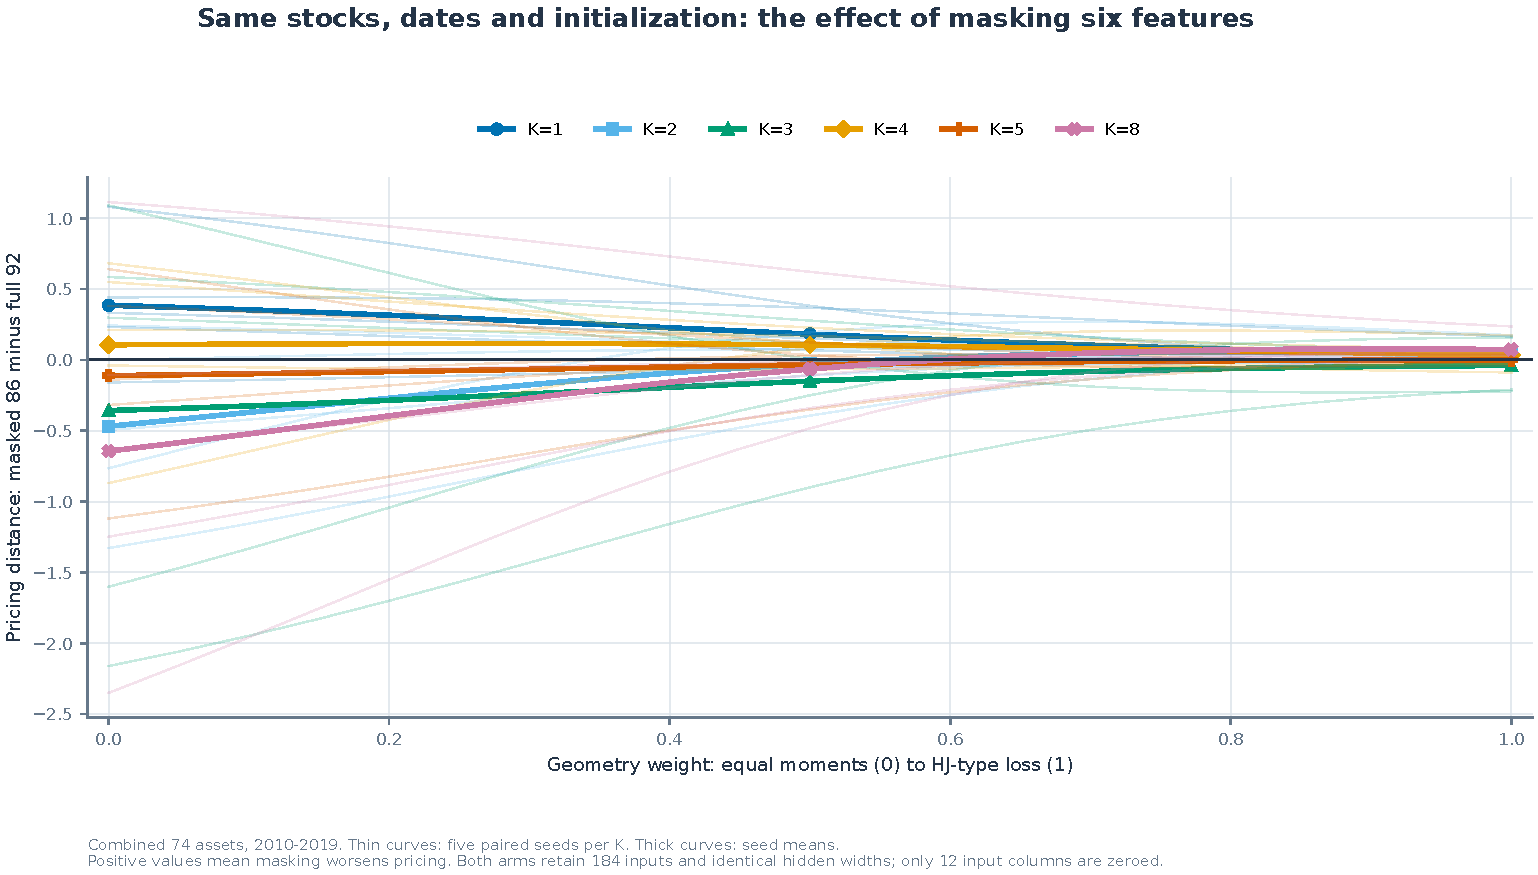
\includegraphics[width=0.98\textwidth]{figure_08_matched_feature_control.pdf}
\caption{Same-panel six-feature ablation for the combined 74 assets. Every curve is a paired difference, masked minus full, on the same 2010--2019 target-return months. Thin lines show all five paired seeds for each fixed $K$; thick lines show their means over the 21 prespecified geometry weights. Positive values mean that masking worsens pricing distance. Both arms have 184 input positions and 128--64--32 hidden widths; only the six characteristic columns and their six missingness indicators are zeroed in the masked arm. The endpoint block-bootstrap intervals are in Table~\ref{tab:matched-features}; thin-line dispersion is algorithmic variation, not a confidence band.}
\label{fig:matched-features}
\end{widefigure}

The control changes the attribution, not the original archived numbers. The historical pipeline reversal cannot be read as a six-characteristic effect. Reconstruction, coverage, timing, and the different input parameterization remain bundled in that older comparison. The present experiment does not decompose their contributions. Its narrower result is that the information deletion tested here leaves endpoint winners for the combined assets unchanged while affecting candidate margins and some intermediate rankings. Geometry dependence persists within both matched arms, without identifying a structural risk count.

% IREF working fragment, 2026-10-06. Not a standalone submission manuscript.
% Sources: P1-G4-V003-R001; calibration qualification P1-G4-V004-R001.
\subsection{Conditional-autoencoder control and the interpretation of dimension}
\label{sec:cae-control}

To assess whether the earlier diagnostic findings extend to a model with more
favorable benchmark performance, we added a conditional-autoencoder control and
a matched linear-loading arm. This extension was specified after the original
study and uses familiar historical data; it is exploratory. The models use 92
ranked characteristics and candidate factor counts $K\in\{1,2,3,4,5,8\}$.
The training, validation, and development periods are August 1963--December 1999,
2000--2009, and 2010--2019, respectively. The extension does not access 2020--2025.
For each architecture, factor count, and initialization, validation reconstruction
loss selects the epoch and one of two regularization settings. Five initializations
produce 120 candidate fits and 60 selected models across the two architectures.
This is a conditional-autoencoder benchmark implementation, not an exact
replication of a published model.

The forecasting exercise uses fixed estimated loadings and expanding factor means
formed from strictly earlier observations. Contemporaneous factors are used for
reconstruction and pricing evaluation, not for forecasting the same month's
returns. SDF coefficients and regularized pricing weights are estimated using
validation data and held fixed in the development evaluation. The reported
pricing norm is HJ-type: it uses the study's regularization and normalization,
so its numerical scale should not be compared directly with differently
normalized HJ distances in other studies.

Validation predictive $R^2$ selects $K=8$ for the conditional autoencoder. Its
validation predictive $R^2$ is 0.0781\%, and its development predictive $R^2$ is
0.2687\%. Its development pricing distance on the combined 74-asset set is
5.0254, compared with 5.9582 for FF5 plus momentum. These point estimates satisfy
the prespecified diagnostic criteria of positive predictive $R^2$ in both periods
and a development pricing distance no larger than the reference. They do not
constitute a statistical noninferiority test or establish superiority over either
the reference factors or the matched linear-loading arm.

Table~\ref{tab:cae-candidates} retains every candidate in both arms. At $K=8$, the linear-loading model has development predictive $R^2$ of 0.2963\%, slightly above the conditional autoencoder, while its pricing distance is 5.1674. These different orderings preclude a general claim of nonlinear-model dominance.

\begin{widetable}[!tbp]
\centering
\caption{Conditional-autoencoder extension: complete development-period candidate comparison}
\label{tab:cae-candidates}
\small
\begin{threeparttable}
\begin{tabular}{@{}r rrr rrr@{}}
\toprule
& \multicolumn{3}{c}{Linear loadings} & \multicolumn{3}{c}{Conditional autoencoder} \\
\cmidrule(lr){2-4}\cmidrule(lr){5-7}
$K$ & Predictive $R^2$ & Pricing distance & Win frequency & Predictive $R^2$ & Pricing distance & Win frequency \\
& (\%) & & (\%) & (\%) & & (\%) \\
\midrule
1 & 0.1555 & 6.0417 & 6.40 & 0.1375 & 6.0127 & 2.05 \\
2 & 0.1594 & 6.3576 & 0.00 & 0.1973 & 6.0961 & 0.05 \\
3 & 0.2323 & 6.1573 & 0.05 & 0.2269 & 5.9433 & 3.95 \\
4 & 0.2880 & 5.3790 & 9.50 & 0.2327 & 5.9172 & 0.40 \\
5 & 0.2903 & 5.2380 & 34.32 & 0.2513 & 5.5869 & 6.35 \\
8 & 0.2963 & 5.1674 & 49.72 & 0.2687 & 5.0254 & 87.19 \\
\bottomrule
\end{tabular}
\begin{tablenotes}[flushleft]\footnotesize
\item Development period: 2010--2019, 120 months and 444,538 stock-months. Pricing uses the combined 74 assets with validation-fixed weights and SDF coefficients. FF5 plus momentum has pricing distance 5.9582 under the same protocol. Each candidate aggregates five selected initializations. Win frequencies use 1,999 common time-block and seed-resampling draws within each architecture; they are descriptive frequencies, not structural-dimension probabilities. No confidence interval or significance ranking is asserted by this table. $K=8$ is the upper endpoint of the prespecified grid. Raw distances are not directly comparable with those from the earlier evaluation-weighted diagnostic protocol.
\end{tablenotes}
\end{threeparttable}
\end{widetable}


Dimension selection is comparatively concentrated in this extension. Under the
prespecified joint time-block and initialization resampling, $K=8$ attains the
smallest development pricing distance in 87.19\% of draws. This is a descriptive
frequency under that resampling procedure, not a probability that the economy
has eight priced shocks. Moreover, eight is the upper endpoint of the fixed
candidate grid. The result qualifies any general statement that these models
necessarily produce unstable dimension choices. It establishes neither a global
optimum over factor counts nor a structural factor dimension.

All 15 pairwise dimension intervals from the exploratory simultaneous procedure
include zero. We do not interpret this as evidence of equivalence or structural
nonidentification. A subsequent, bounded known-truth calibration of that procedure
found simultaneous coverage of 83.5\% and 87.0\%, below the nominal 95\%, in its two
primary 120-month equal-distance scenarios. \ref{app:inference-calibration}
reports the design and results. Accordingly, the intervals remain an archived
exploratory output rather than a calibrated confidence set for dimension.
The separate pointwise forecasting and benchmark-comparison intervals were not
validated by that calibration either; the extension's substantive comparison is
therefore limited to the reported point estimates and descriptive selection
behavior.

The control separates a model's observed performance from the interpretation of
its selected width. It supplies a case with favorable point-estimate diagnostics
and comparatively concentrated selection, alongside the earlier diagnostic
family. The combined evidence does not establish that successful pricing models
share an unstable economic structure. Rather, claims about economic dimension
require an identified economic object and evidence beyond the fitted width,
activation rank, or minimum of a finite candidate loss grid.


\subsection{External assets and the common market direction}

In the development period, Core-86 changes best dimension between geometry endpoints for all six external families, but its raw contrast statistic $A$ has a bootstrap interval containing zero in every family. The market-direction attenuation point estimate is positive for five of six families, yet all six intervals contain zero. Adding the market factor to $K=1$ improves raw Euler moments with intervals excluding zero in five of six families, while alpha improvement excludes zero in none. Under Core-92, the same diagnostics appear much stronger: $A$, raw-moment completion, and alpha completion exclude zero for all six families. This difference shows sensitivity between the archived pipelines, which also differ in coverage and timing; it cannot be attributed to data construction alone.

The spectral decomposition provides a coherent economic clue. Compression loss is concentrated in a small number of high-variance common directions. The largest spectral direction is close to the equal-weighted payoff direction, and hedging assets by validation-period market betas reduces the point-estimate geometry contrast. A compact representation can therefore recover aggregate market variation while losing finer relative-pricing information. Adding the market factor can repair a dominant unconditional Euler direction without repairing the cross-section of alphas.

That distinction answers why the direction of compression matters. The decomposition localizes part of the observed error contrast to common payoff variation. It does not establish which information is lost first inside the network, nor identify a causal effect of compression. The absence of joint alpha improvement limits the interpretation to the reported diagnostics.

\subsection{The locked 2020--2025 test}

The development-period dimension pattern does not persist in the locked period (Figure~\ref{fig:sealed-dashboard}). Reading across a row connects endpoint dimension, the raw geometry contrast, market-direction attenuation, raw-moment completion, and alpha completion; hollow diamonds and arrows add the development estimate wherever the same external family is available. Seven of nine asset sets select $K=1$ at both endpoints. Size--accruals and size--residual-variance select $K=1$ under equal moments and $K=8$ under HJ. Combined 74 selects $K=1$ under both. This is a much more uniformly low-dimensional period than development.

\begin{widefigure}[!tbp]
\centering
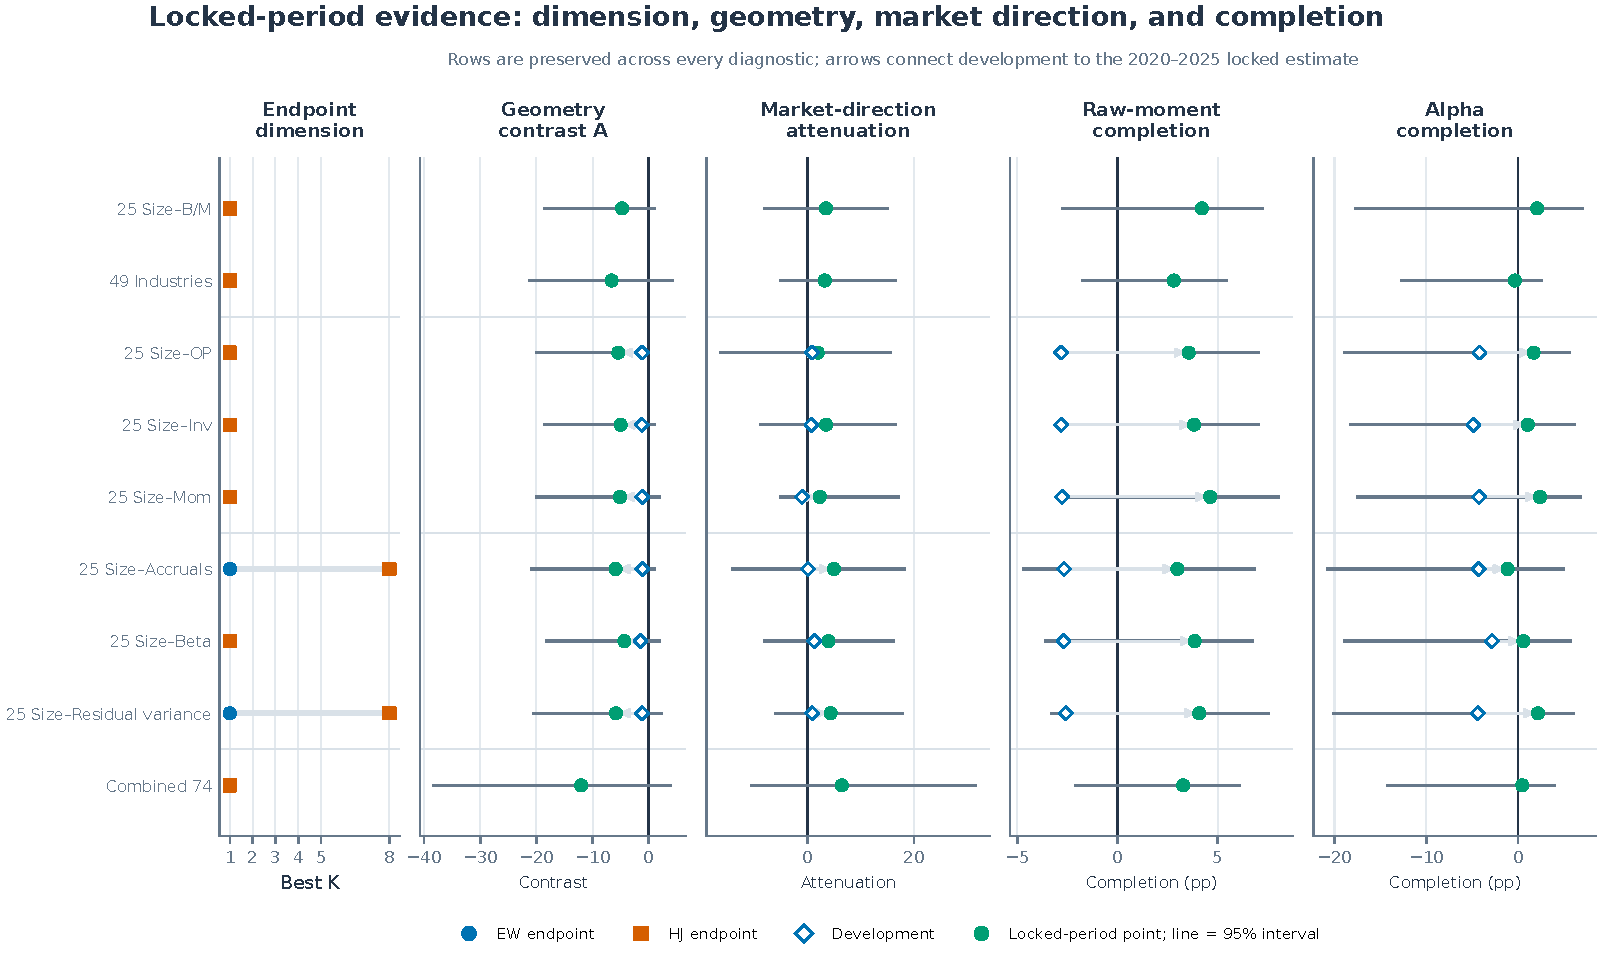
\includegraphics[width=0.99\textwidth]{figure_04_sealed_falsification.pdf}
\caption{Asset-aligned locked 2020--2025 evidence field. Each row preserves one test-asset family across endpoint dimension, raw geometry contrast $A$, market-direction attenuation, raw-moment completion, and alpha completion. Green points and horizontal lines report the locked estimate and its 95\% circular-block interval. For the six external families, hollow diamonds mark the development estimate and arrows point to the locked estimate. The first track compares equal-moment and HJ endpoint dimensions. The Core-86 models and rules were fixed before this later evaluation. Earlier legacy development includes January 2020; the period is not a wholly untouched research holdout.}
\label{fig:sealed-dashboard}
\end{widefigure}

Table~\ref{tab:sealed-evidence} places each asset family's selected dimensions beside its pricing diagnostics and 95\% intervals. The locked point estimates have the anticipated market-attenuation sign but do not provide precise evidence of that effect or confirm the broader dimension pattern. The four frozen decisions follow directly from these rows. Geometry dependence fails because only two of six external families change endpoint dimension, below the four-family threshold, and Combined 74 does not change. The market-direction gate passes its point-estimate rule: attenuation is positive for Combined 74 and all six external families. Precision is limited because every corresponding block-bootstrap interval contains zero. Economic completion fails: no external family jointly improves raw moments and alpha. Dimension diversity fails because only $K=1$ and $K=8$ appear among external endpoint winners.



\begin{widetable}[!tbp]
\centering
\begin{minipage}{\textwidth}
\caption{Pricing dimensions and economic diagnostics in the locked 2020--2025 evaluation}
\label{tab:sealed-evidence}
\footnotesize
\setlength{\tabcolsep}{4pt}
\renewcommand{\arraystretch}{1.16}
\begin{tabular*}{\linewidth}{@{\extracolsep{\fill}}lccrrrr@{}}
\toprule
Test assets & \multicolumn{2}{c}{Best $K$} & Geometry & Market & \multicolumn{2}{c}{Completion (pp)} \\
\cmidrule(lr){2-3}\cmidrule(l){6-7}
 & EW & HJ & contrast $A$ & attenuation & Raw moments & Alpha \\
\midrule
\multicolumn{7}{@{}l}{\textit{Primary assets}} \\[2pt]
Size--B/M & 1 & 1 & -4.76 & 3.52 & 4.21 & 2.09 \\
 &  &  & [-18.76, 1.12] & [-8.15, 15.30] & [-2.80, 7.26] & [-17.85, 7.13] \\
Industries & 1 & 1 & -6.62 & 3.28 & 2.81 & -0.34 \\
 &  &  & [-21.32, 4.45] & [-5.11, 16.68] & [-1.82, 5.46] & [-12.85, 2.65] \\
Combined 74 & 1 & 1 & -12.04 & 6.48 & 3.28 & 0.48 \\
 &  &  & [-38.52, 4.11] & [-10.68, 31.74] & [-2.15, 6.16] & [-14.34, 4.10] \\
\addlinespace[4pt]
\multicolumn{7}{@{}l}{\textit{External assets}} \\[2pt]
Size--OP & 1 & 1 & -5.42 & 1.97 & 3.55 & 1.71 \\
 &  &  & [-20.16, -1.57] & [-16.47, 15.77] & [-3.06, 7.07] & [-19.07, 5.73] \\
Size--Inv & 1 & 1 & -5.00 & 3.54 & 3.82 & 1.07 \\
 &  &  & [-18.79, 1.11] & [-8.88, 16.66] & [-3.03, 7.06] & [-18.41, 6.27] \\
Size--Mom & 1 & 1 & -5.12 & 2.37 & 4.62 & 2.41 \\
 &  &  & [-20.16, 2.02] & [-5.11, 17.40] & [-2.94, 8.10] & [-17.58, 6.94] \\
Size--Accruals & 1 & 8 & -5.90 & 4.99 & 2.99 & -1.13 \\
 &  &  & [-20.99, 1.15] & [-14.19, 18.37] & [-4.73, 6.89] & [-20.89, 5.05] \\
Size--Beta & 1 & 1 & -4.36 & 3.97 & 3.85 & 0.59 \\
 &  &  & [-18.32, 2.14] & [-8.28, 16.33] & [-3.66, 6.78] & [-18.99, 5.86] \\
Size--Residual var. & 1 & 8 & -5.84 & 4.40 & 4.07 & 2.18 \\
 &  &  & [-20.71, 2.36] & [-6.18, 18.08] & [-3.35, 7.59] & [-20.26, 6.21] \\
\bottomrule
\end{tabular*}
\par\vspace{4pt}
{\footnotesize\raggedright\textit{Notes:} Brackets below each diagnostic are 95\% twelve-month circular-block bootstrap intervals (500 draws). Positive market attenuation means hedging reduces the absolute geometry contrast. Completion is the error of $K=1$ plus the market factor minus the error of $K=1$, multiplied by 100; negative values indicate improvement. EW and HJ denote the equal-moment and covariance-weighted endpoints. All rows use the frozen Core-86 models.\par}
\end{minipage}
\end{widetable}


The locked result narrows the interpretation of development evidence. Development evidence suggested broad geometry dependence. The locked period says that this pattern is not stable; one factor ranks first for most evaluated spans under the fixed models. This ranking alone does not identify a change in the economy's true risk count. The market-direction clue is more persistent in sign than the exact dimension ranking, but its uncertainty is too large for a strong structural claim. The last two tracks of Figure~\ref{fig:sealed-dashboard} make the development-to-locked completion reversal visible row by row across the six external families.

\subsection{Known-truth evidence on exact dimension recovery}

Feasible evaluation recovers the true dimension much less often than oracle evaluation. Table~\ref{tab:sim-mechanisms} separates the marginal selection frequencies (Panel A) from the eight prespecified mechanism contrasts (Panel B). All eight contrasts have the planned sign. Overall exact recovery is 64.2\% under oracle evaluation and 32.6\% under feasible evaluation. Increasing the sample from 72 to 600 months raises recovery from 38.1\% to 58.2\%, but the gain combines oracle and feasible designs and does not eliminate feasible over-selection. Strong risk prices raise recovery by 23.0 percentage points relative to weak prices. Full spanning raises it by 12.0 points relative to weak-tail spanning.

\begin{widetable}[!tbp]
\centering
\begin{minipage}{\textwidth}
\caption{Known-truth dimension selection: outcomes and prespecified mechanism contrasts}
\label{tab:sim-mechanisms}
\footnotesize
\setlength{\tabcolsep}{4pt}
\renewcommand{\arraystretch}{1.16}
\begin{tabular*}{\linewidth}{@{\extracolsep{\fill}}llrrrr@{}}
\toprule
\multicolumn{6}{@{}l}{\textit{A. Marginal selection outcomes}} \\[2pt]
Design axis & Level & Exact (\%) & Under (\%) & Over (\%) & Mean error \\
\midrule
Evaluation & Feasible & 32.6 & 33.9 & 33.5 & 1.693 \\
 & Oracle & 64.2 & 35.8 & 0.0 & 0.760 \\
\addlinespace[2pt]
Sample months & 72 & 38.1 & 46.2 & 15.7 & 1.526 \\
 & 240 & 48.9 & 34.4 & 16.8 & 1.197 \\
 & 600 & 58.2 & 23.9 & 17.8 & 0.956 \\
\addlinespace[2pt]
Risk prices & Strong & 59.9 & 22.1 & 17.9 & 0.900 \\
 & Weak & 36.9 & 47.5 & 15.6 & 1.552 \\
\addlinespace[2pt]
Asset spanning & Full & 54.4 & 28.6 & 16.9 & 1.105 \\
 & Weak tail & 42.4 & 41.0 & 16.6 & 1.347 \\
\addlinespace[2pt]
True dimension & 1 & 74.2 & 0.0 & 25.8 & 0.775 \\
 & 3 & 38.0 & 44.9 & 17.1 & 1.120 \\
 & 5 & 33.1 & 59.5 & 7.4 & 1.784 \\
\addlinespace[2pt]
Test assets & 25 & 46.8 & 36.7 & 16.5 & 1.257 \\
 & 74 & 50.0 & 33.0 & 17.0 & 1.195 \\
\addlinespace[2pt]
Factor correlation & 0.0 & 47.0 & 36.8 & 16.2 & 1.259 \\
 & 0.7 & 49.8 & 32.9 & 17.3 & 1.194 \\
\addlinespace[2pt]
Pricing geometry & Equal moments & 46.7 & 35.1 & 18.2 & 1.337 \\
 & HJ & 50.2 & 34.5 & 15.3 & 1.116 \\
\bottomrule
\end{tabular*}
\par\vspace{7pt}
\begin{tabular*}{\linewidth}{@{\extracolsep{\fill}}lrrr@{}}
\toprule
\multicolumn{4}{@{}l}{\textit{B. Prespecified mechanism contrasts}} \\[2pt]
Contrast and outcome & Cells & Effect (pp) & 95\% cell interval (pp) \\
\midrule
More time: exact recovery$^{a}$ & 24 & 26.5 & [17.8, 35.2] \\
Strong minus weak prices: exact recovery & 288 & 23.0 & [20.3, 25.7] \\
Weak minus strong prices: under-selection & 288 & 25.4 & [22.7, 28.1] \\
Full minus weak-tail span: exact recovery & 288 & 12.0 & [10.4, 13.6] \\
Weak-tail minus full span: asset-family divergence & 288 & 7.4 & [5.2, 9.6] \\
Equal--HJ disagreement: level$^{b}$ & 288 & 20.3 & [17.7, 22.9] \\
Complex minus baseline designs: disagreement$^{c}$ & 216 & 22.9 & [20.0, 25.9] \\
Oracle minus feasible evaluation: exact recovery & 288 & 31.6 & [29.0, 34.2] \\
\bottomrule
\end{tabular*}
\par\vspace{4pt}
{\footnotesize\raggedright\textit{Notes:} Panel A averages the remaining frozen design axes; its rows do not hold every other axis fixed. Exact, under-, and over-selection sum to 100\% before rounding; mean error is $|\widehat K-K_0|$. Oracle over-selection is zero by construction. Panel B uses percentage points (pp). Its archived intervals are the mean $\pm1.96$ standard errors across design-cell contrasts; they summarize cell heterogeneity, not uncertainty from independent Monte Carlo draws. $^{a}$600 minus 72 months, restricted to strong prices, full span, and $\rho=0$. $^{b}$An average level, not a difference. $^{c}$Correlation and/or weak-tail designs relative to full spanning with $\rho=0$. There are 500 Monte Carlo repetitions per base condition; six asset families share each repetition.\par}
\end{minipage}
\end{widetable}


Figure~\ref{fig:identification-dashboard} shows how recovery changes with sample length within each design. Panels A--B retain joint conditioning: rows separate risk-price strength and asset spanning, colors identify the true dimension, and line styles separate oracle from feasible evaluation. In the most favorable strong-price, full-span, zero-correlation design, oracle recovery at $T=600$ is 100\% for $K_0=1$, 99.8\% for $K_0=3$, and 99.2\% for $K_0=5$. These cells illustrate substantially better recovery when the evaluation mean is known. Feasible selection behaves differently. For $K_0=1$, recovery is approximately 46--51\% across 72, 240, and 600 months under the two geometries. Its over-selection probability does not vanish.

\begin{widefigure}[!tbp]
\centering
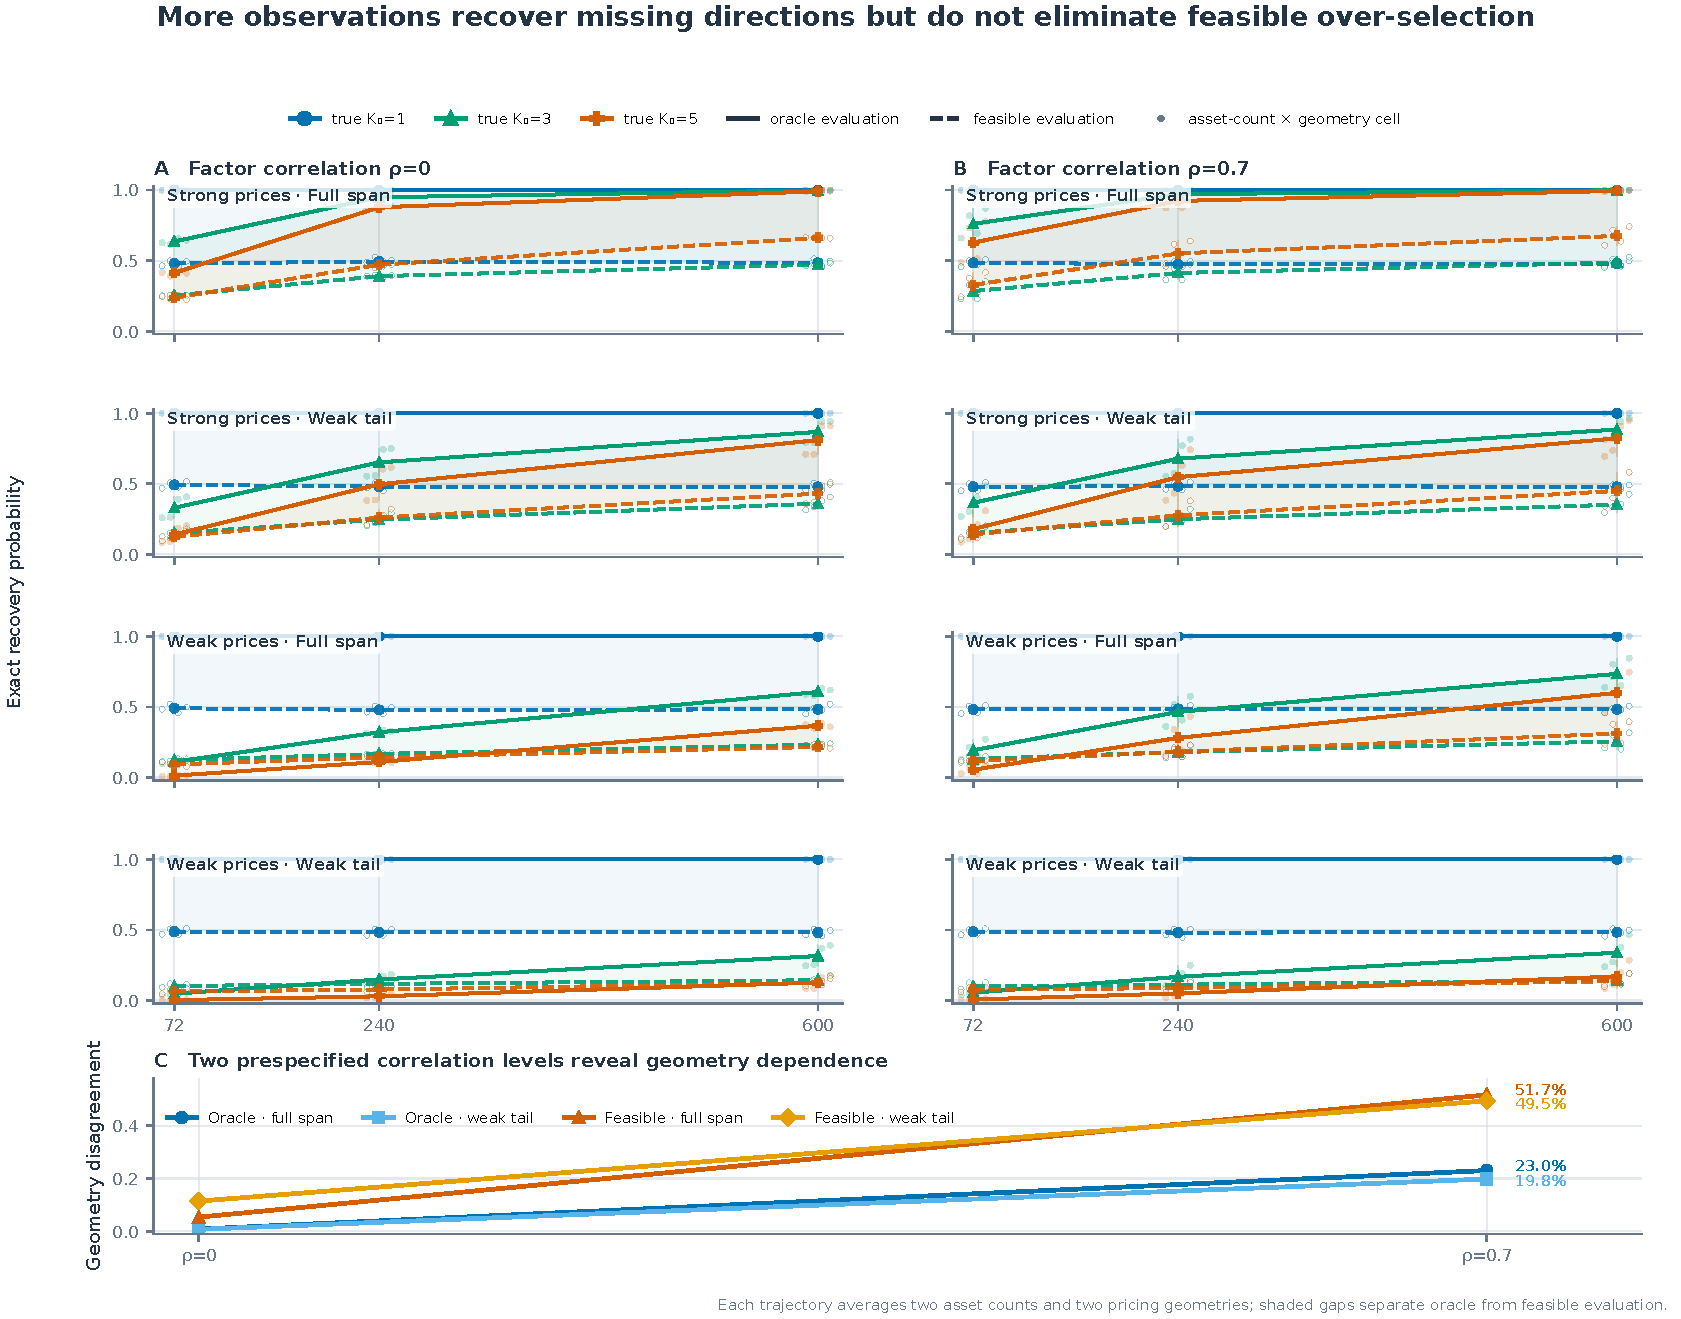
\includegraphics[width=0.99\textwidth]{figure_05_identification_mechanisms.pdf}
\caption{Known-truth identification trajectories over the complete frozen condition grid. Panels A and B plot exact recovery at the three prespecified sample lengths, 72, 240, and 600 months, under factor correlations zero and 0.7. Rows distinguish risk-price strength and asset spanning; colors identify $K_0$; solid and dashed lines separate oracle and feasible evaluation. Small points expose the four asset-count--pricing-geometry cells behind each mean marker; their vertical range is also shown. Each mean is therefore based on 12,000 selection outcomes. Shaded gaps show the loss from feasible evaluation. Panel C is a two-level slope graph, rather than an interpolated correlation curve, and reports equal-versus-HJ dimension disagreement at the two prespecified correlation values.}
\label{fig:identification-dashboard}
\end{widefigure}

The result illustrates Proposition~\ref{prop:inconsistency}. Models above $K_0$ add directions with zero population price. Their empirical losses fluctuate around the same population value, so the strict minimum rewards whichever redundant direction happens to reduce sample loss. More data shrink all differences, but they do not force the sign of a centered, second-order difference to favor the minimal model. In the aggregate feasible design, the over-selection rate is 33.5\%; it rises from 31.3\% at 72 months to 35.7\% at 600 months rather than disappearing.

\subsection{Asset spanning and geometry disagreement}

Weak-tail spanning reduces the loadings on the final true directions to 0.15 of their baseline magnitude. Exact recovery falls by 12.0 percentage points, and the probability that six asset families select different dimensions rises by 7.4 points. Under oracle evaluation, multiple dimensions appear across the six families in 27.8\% of strong/full conditions, 55.1\% of strong/weak-tail conditions, and about 63--65\% of weak-price conditions. Under feasible evaluation, cross-family diversity appears in 98--99\% of conditions. A common economic dimension can therefore generate heterogeneous empirical dimensions when assets reveal its weaker directions unevenly.

Equal and HJ geometries disagree on the selected dimension in 20.3\% of all simulation cases. With independent factor directions and full spanning, disagreement is only 0.8\% under oracle evaluation and 5.3\% under feasible evaluation. Raising factor correlation to 0.7 increases those rates to 23.0\% and 51.7\%. Panel C of Figure~\ref{fig:identification-dashboard} displays this amplification.

The simulation does not identify which mechanism causes each empirical result. It establishes that the specified combinations of weak prices, weak spanning, correlated risks, weighting, and evaluation noise can generate unstable selection. The design contrasts do not imply that each mechanism alone explains the empirical results. It would be invalid to invert the simulation and declare the true empirical dimension or the causal share of each mechanism.

\subsection{Descriptive loss-tolerance sets}

A candidate minimum can be accompanied by a transparent loss-tolerance set,
\begin{equation}
 \widehat{\mathcal A}_{\delta}^{\mathrm{desc}}=
 \{K:\widehat\Loss(K)-\min_j\widehat\Loss(j)\leq\delta\}.
\end{equation}
Here $\delta$ is a stated descriptive tolerance, not a critical value. This set
reports proximity to the observed minimum. It is neither a confidence set for
the population minimizer nor evidence of statistical or economic equivalence.
The conditional-autoencoder archive uses a fixed tolerance of 1\% of the
FF5-plus-momentum development distance and retains the full candidate losses.
That convention has no claim to being a universally appropriate economic
threshold. A formal equivalence claim would require a justified margin and
valid uncertainty assessment for the corresponding estimand. The failed
calibration in \ref{app:inference-calibration} prevents the new
simultaneous intervals from supplying that assessment here.
